\documentclass[12pt, twoside]{article}
\usepackage{amsmath}
\usepackage{tikz}
\usetikzlibrary{calc, patterns}
\usepackage{caption}
\usepackage[marginparwidth=5cm, marginparsep=0.5cm,
top=4cm, bottom=4cm, left=2.5cm, right=6.5cm]{geometry}
\usepackage[latin]{babel}
\usepackage{amsfonts}
\newcommand{\Identity}{\mathbb{I}}
\newcommand{\matgg}{\vec{\gamma}}
\newcommand{\TimeDerivative}{\dot}
\newcommand{\of}[1]{(#1)}


\usepackage[iso]{datetime}
\usepackage{hyperref}

\begin{document}
\newcommand{\FigureSimplePendulumConfigurationSpace}{%
\begin{tikzpicture}
%\draw [fill, pattern = north east lines, draw = none] (-1.75, 0) -- ++(3.5, 0) -- ++(45:.25) -- ++(-3.5, 0) -- cycle;
\useasboundingbox (-2.5, -4) rectangle (2.5, 0);
\foreach \x in {-.5,-.45,...,.51}
  \draw (\x, 0) -- ++(45:.125);
\draw (-.5, 0) -- (.5, 0);
\coordinate (P) at (0, 0);
\coordinate (I) at (0, -4);
\node at (-65 : 4) [name=m, circle, inner sep = .25 cm, draw] {};
\node at (P) [name=pivot, label={[label distance=1cm]-87:$q$}] {};
\draw (P) -- (m);
\draw [->] (-90 : 1) arc (-90 : -65 : 1);
\draw [dashdotted] (I) -- (P);
\end{tikzpicture}%
}

\newcommand{\FigureDoublePendulumConfigurationSpace}{%
\begin{tikzpicture}
%\draw [fill, pattern = north east lines, draw = none] (-1.75, 0) -- ++(3.5, 0) -- ++(45:.25) -- ++(-3.5, 0) -- cycle;
%\foreach \x in {-1.75,-1.65,...,1.76}
%  \draw (\x, 0) -- ++(45:.25);
%\draw (-1.75, 0) -- (1.75, 0);
\useasboundingbox (-2.5, -4) rectangle (2.5, 0);
\foreach \x in {-.5,-.45,...,.51}
  \draw (\x, 0) -- ++(45:.125);
\draw (-.5, 0) -- (.5, 0);
\coordinate (P) at (0, 0);
\coordinate (I) at (0, -4);
\coordinate (M1) at (-60 : 2);
\coordinate (M2) at ($(M1) + (-150 : 2)$);
\coordinate (D) at ($(M1)-(P)!(M1)!(I)$);
\coordinate (I2) at ($(I)+(D)$);
\node at (M1) [name=m1, circle, inner sep = .125 cm, label={[label distance=1cm]-100:$q_2$}, draw] {};
\node at (M2) [name=m2, circle, inner sep = .125 cm, draw] {};
\node at (P) [name=pivot, label={[label distance=1cm]-87:$q_1$}] {};
\draw (P) -- (m1) -- (m2);
\draw [->] (-90 : 1) arc (-90 : -60 : 1);
\draw [->] ($(M1)+(0, -1)$) arc (-90 : -150 : 1);
\draw [dashdotted] (I) -- (P);
\draw [dashdotted] (I2) -- (m1);
\end{tikzpicture}
}

\newcommand{\FigureComplexThingThatYouCantVisualise}{%
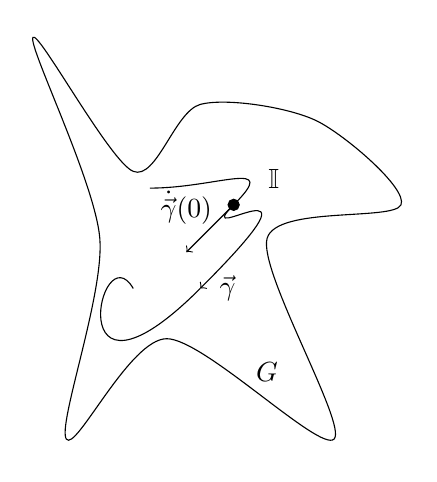
\begin{tikzpicture}[scale=.85]
\coordinate (I) at (.5,.5);
\coordinate (Tin) at (45:1);
\coordinate (Tout) at (45:-1);
\coordinate (P) at (0,-.75);
\coordinate (Pin) at (45:3);
\coordinate (Pout) at (45:-3);
\draw plot [smooth cycle] coordinates {(1.75,1.75) (0,2) (-1,1) (-2.5,3) (-1.5,0) (-2,-3) (-.5,-1.5) (2,-3) (1,0) (3,.5)};
\node at (I) [name=i, circle, inner sep = .05 cm, fill=black, label={[label distance=0.25cm]15:$\Identity$}, draw] {};
\node at ($(I)+(Tout)$) [name=t, label={[label distance = 0.1 cm]90:$\TimeDerivative\matgg\of 0$}] {};
\draw [->] (I) -- +(Tout);
\node at (P) [name=p, label={0:$\matgg$}] {};
\draw (-.75,.75) .. controls +(0:1) and +(Tin)  .. (I);
\draw [->] (I) .. controls +(Tout) and +(Pin) .. (P);
\draw (P) .. controls +(Pout) and +(120:1) .. (-1,-.75);
\node at (1, -2) {$G$};
\end{tikzpicture}%
}%
\noindent
\today T\currenttime
\section*{Catilina pendulaque}
Quousque tandem abutere, Catilina, patientia nostra? quamdiu etiam furor iste tuus nos eludet? quem ad finem sese effrenata jactabit audacia? Nihilne te nocturnum praesidium Palati, nihil urbis vigiliae, nihil timor populi, nihil concursus bonorum omnium, nihil hic munitissimus habendi senatus locus, nihil horum ora voltusque moverunt? Patere tua consilia non sentis, constrictam jam horum omnium scientia teneri conjurationem tuam non vides? Quid proxima, quid superiore nocte egeris, ubi fueris, quos convocaveris, quid consilii ceperis, quem nostrum ignorare arbitraris?
\marginpar{
\FigureSimplePendulumConfigurationSpace%
\captionof{figure}{Simplex pendula massa.}
}

O tempora, o mores! Senatus haec intellegit. Consul videt; hic tamen vivit. Vivit? immo vero etiam in senatum venit, fit publici consilii particeps, notat et designat oculis ad caedem unum quemque nostrum. Nos autem fortes viri satisfacere rei publicae videmur, si istius furorem ac tela vitemus. Ad mortem te, Catilina, duci iussu consulis iam pridem oportebat, in te conferri pestem, quam tu in nos [omnes iam diu] machinaris.

An vero vir amplissumus, P. Scipio, pontifex maximus, Ti. Gracchum mediocriter labefactantem statum rei publicae privatus interfecit; Catilinam orbem terrae caede atque incendiis vastare cupientem nos consules perferemus? Nam illa nimis antiqua praetereo, quod C. Servilius Ahala Sp.\ Maelium novis rebus studentem manu sua occidit. Fuit, fuit ista quondam in hac re publica virtus, ut viri fortes acrioribus suppliciis civem perniciosum quam acerbissimum hostem coercerent. Habemus senatus consultum in te, Catilina, vehemens et grave, non deest rei publicae consilium neque auctoritas huius ordinis; nos, nos, dico aperte, consules desumus.

\begin{figure}
\FigureComplexThingThatYouCantVisualise
\caption{Res.}
\end{figure}

Decrevit quondam senatus, ut L. Opimius consul videret, ne quid res publica detrimenti caperet; nox nulla intercessit; interfectus est propter quasdam seditionum suspiciones C. Gracchus, clarissimo patre, avo, maioribus, occisus est cum liberis M. Fulvius consularis. Simili senatus consulto C. Mario et L. Valerio consulibus est permissa res publica; num unum diem postea L. Saturninum tribunum pl. et C. Servilium praetorem mors ac rei publicae poena remorata est? At [vero] nos vicesimum iam diem patimur hebescere aciem horum auctoritatis. Habemus enim huiusce modi senatus consultum, verum inclusum in tabulis tamquam in vagina reconditum, quo ex senatus consulto confestim te interfectum esse, Catilina, convenit. Vivis, et vivis non ad deponendam, sed ad confirmandam audaciam. Cupio, patres conscripti, me esse clementem, cupio in tantis rei publicae periculis me non dissolutum videri, sed iam me ipse inertiae nequitiaeque condemno.

Castra sunt in Italia contra populum Romanum in Etruriae faucibus conlocata, crescit in dies singulos hostium numerus; eorum\marginpar{
\begin{center}
\FigureDoublePendulumConfigurationSpace%
\captionof{figure}{Duplex pendulae massae.}
\end{center}
} autem castrorum imperatorem ducemque hostium intra moenia atque adeo in senatu videmus intestinam aliquam cotidie perniciem rei publicae molientem. Si te iam, Catilina, comprehendi, si interfici iussero, credo, erit verendum mihi, ne non potius hoc omnes boni serius a me quam quisquam crudelius factum esse dicat. Verum ego hoc, quod iam pridem factum esse oportuit, certa de causa nondum adducor ut faciam. Tum denique interficiere, cum iam nemo tam inprobus, tam perditus, tam tui similis inveniri poterit, qui id non iure factum esse fateatur.
\end{document}